\begin{frame}
    \frametitle{Outline} 
    \tableofcontents[currentsection]
\end{frame} 

\begin{frame}
    \frametitle{Motivation}
    \begin{columns}[onlytextwidth]
        \begin{column}{0.45\textwidth}
            \begin{flushleft}
                \vspace{-1.5cm}
                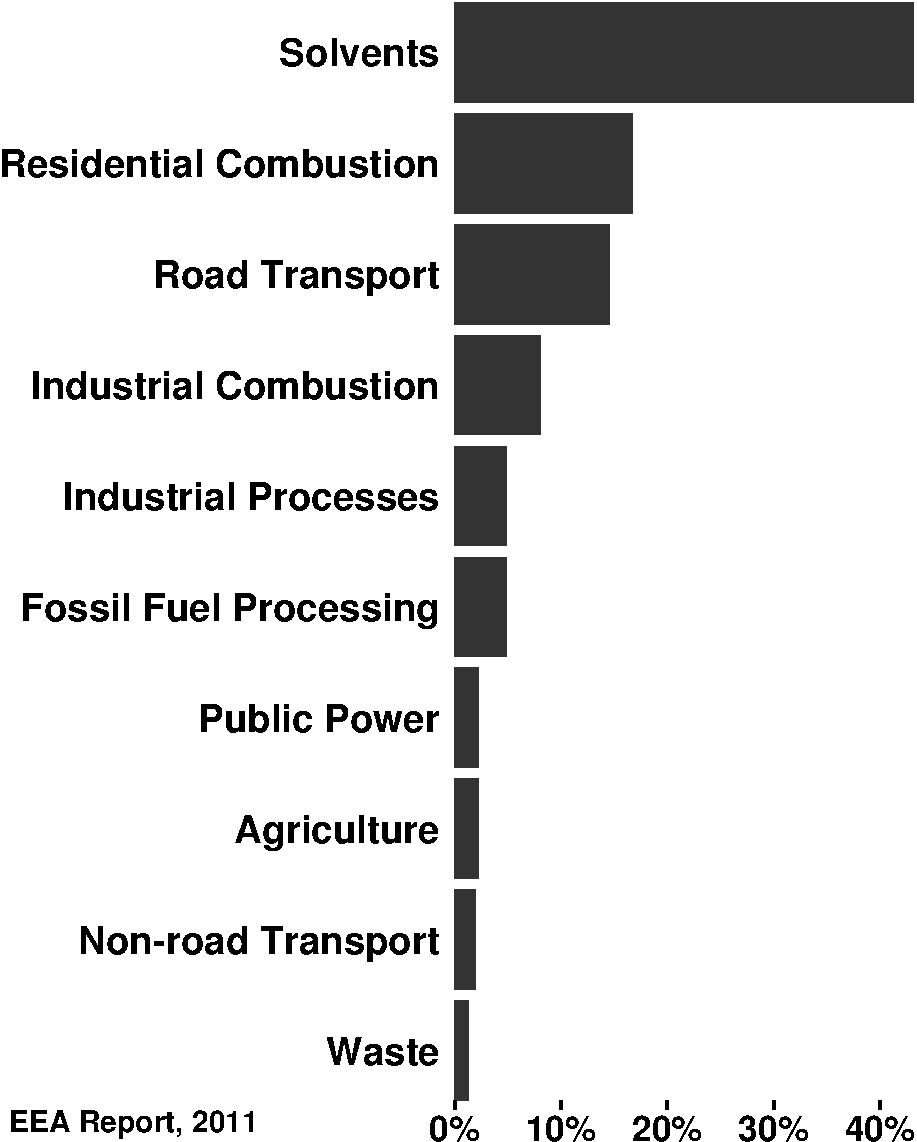
\includegraphics[width=1.10\textwidth]{../Pictures/Sector_conributions} 
            \end{flushleft}
        \end{column}%
        \begin{column}{0.45\textwidth}
            \begin{flushright}
                \vspace{-1.5cm}
                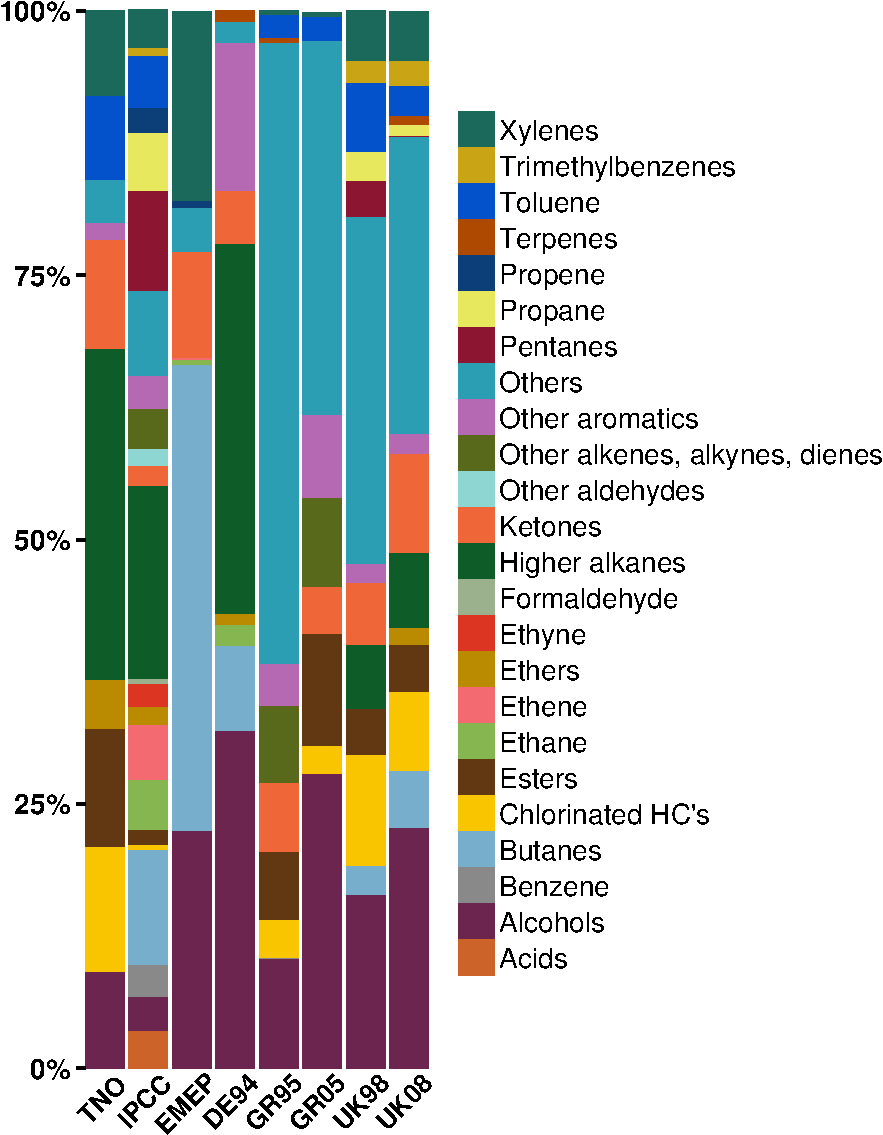
\includegraphics[width=1.10\textwidth]{../Pictures/Speciations_for_MCM} 
            \end{flushright}
        \end{column}
    \end{columns}
\end{frame}

\begin{frame}
    \frametitle{Compared Solvent Speciations}

    \vspace{-0.4cm}
    {
        \setstretch{1.15}
        \begin{table}%[!ht]
            \begin{center}
                \small\makebox[\textwidth][c]{%
                \begin{tabular}{lllP{5.2cm}}
                    \toprule
                    \textbf{Speciation} & \textbf{Reference} \\ \bottomrule
                    TNO & [Builtjes et al., TNO Report, 2002] \\ \hline
                    IPCC & [Ehhalt et al., IPCC Report, 2001] \\ \hline
                    EMEP & [Simpson et al., ACP, 2010] \\ \hline
                    DE94 & [Friedrich et. al., JAC, 2002] \\ \hline
                    GR95 & [Sidiropoulos and Tsilingiridis, FEB, 2007] \\ \hline
                    GR05 & [Sidiropoulos and Tsilingiridis, FEB, 2007] \\ \hline
                    UK98 & [Goodwin, UK NAEI report, 2000] \\ \hline
                    UK08 & [Murrells et al., UK NAEI Report, 2010] \\ \bottomrule
                \end{tabular}}
            \end{center}
        \end{table}
    }
\end{frame}

\begin{frame}
    \frametitle{Boxmodel Setup}

    \vspace{-5mm}
    \begin{itemize}
        \item MECCA boxmodel over 7 days. \vspace{3mm}
        \item Idealised urban area of 1000 km$^2$. \vspace{3mm}
        \item Solvent sector contributes 43 \% to total NMVOC emissions (1000 tons/day) [Warnecke et al., JGR, 2007]. \\ Total NMVOC emissions of 430 tons/day. \vspace{3mm}
        \item NMVOC emissions constant until noon of day 1.\vspace{3mm}
        \item NO source tuned for maximum ozone production. 
    \end{itemize}
\end{frame}

{
    \usebackgroundtemplate{%
        \vbox to \paperheight{\vfil\hbox to \paperwidth{\hfil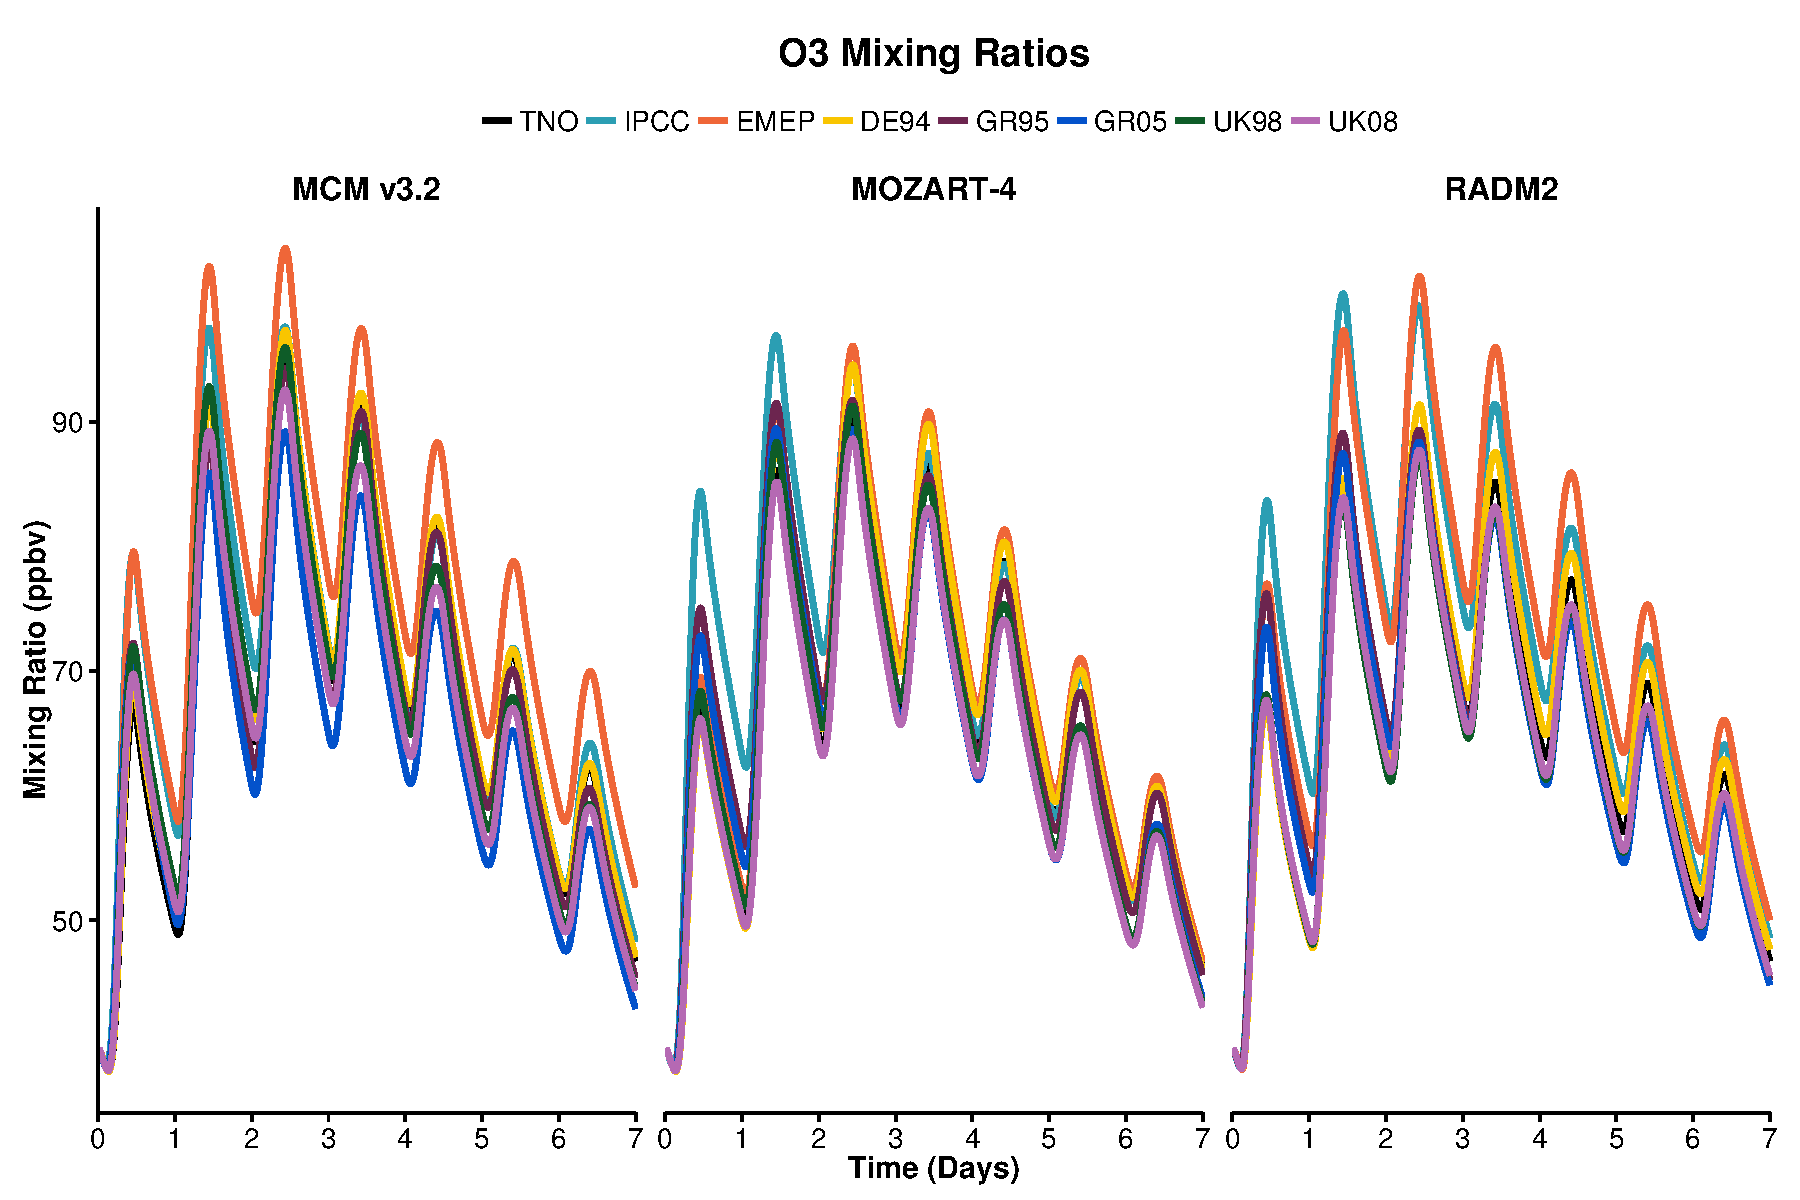
\includegraphics[height=0.70\paperheight, width = 0.95\paperwidth]{../Plotting_scripts/Solvents_Only_O3_mixing_ratios}\hfil}\vfil}
    }
    \begin{frame}[plain]
    \end{frame}
}

{
    \usebackgroundtemplate{%
        \vbox to \paperheight{\vfil\hbox to \paperwidth{\hfil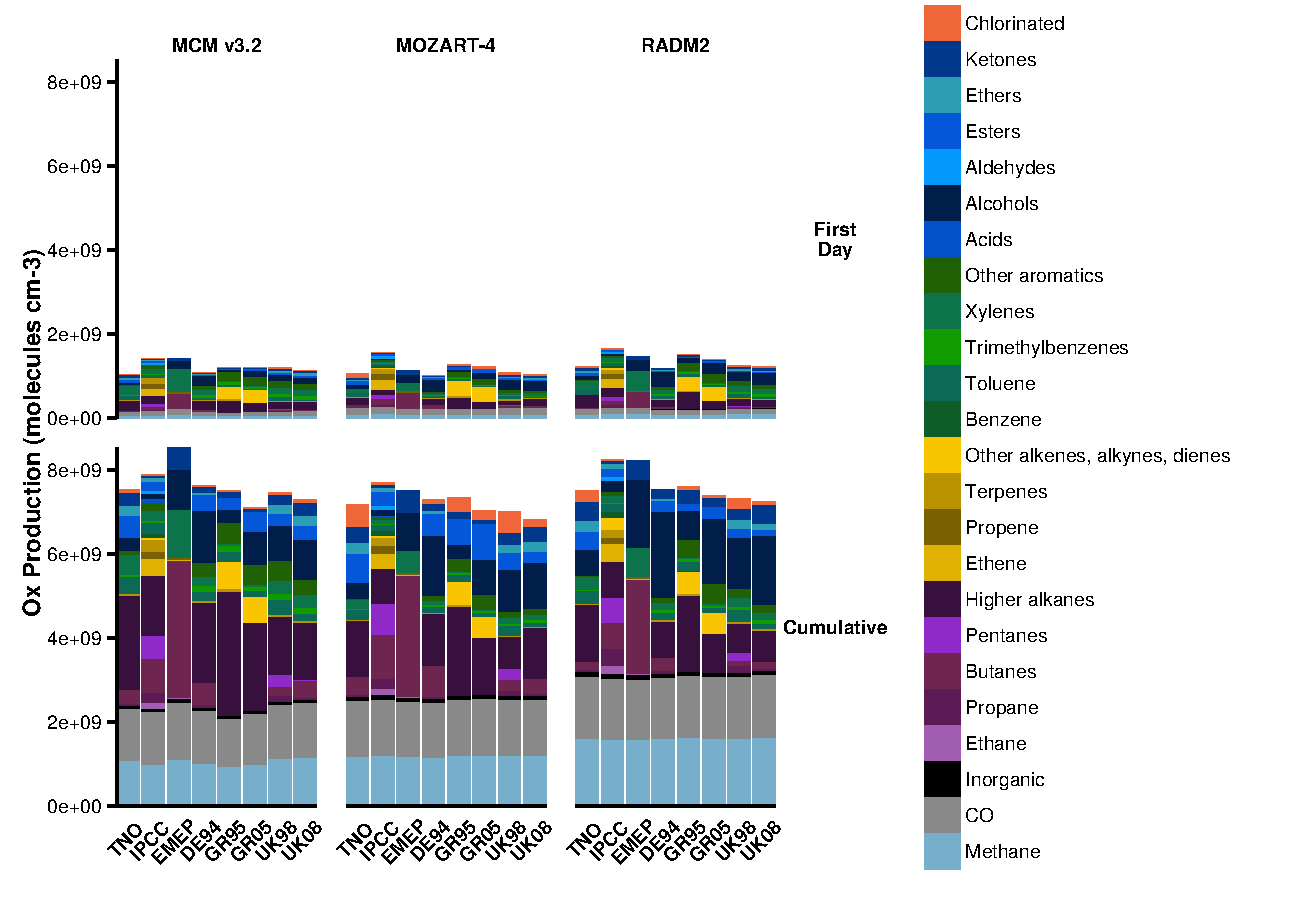
\includegraphics[height=0.90\paperheight, width = 0.98\paperwidth]{../Plotting_scripts/Absolute_Ox_budget_allocated_facet_mechanism}\hfil}\vfil}
    }
    \begin{frame}[plain]
    \end{frame}
}

{
    \usebackgroundtemplate{%
        \vbox to \paperheight{\vfil\hbox to \paperwidth{\hfil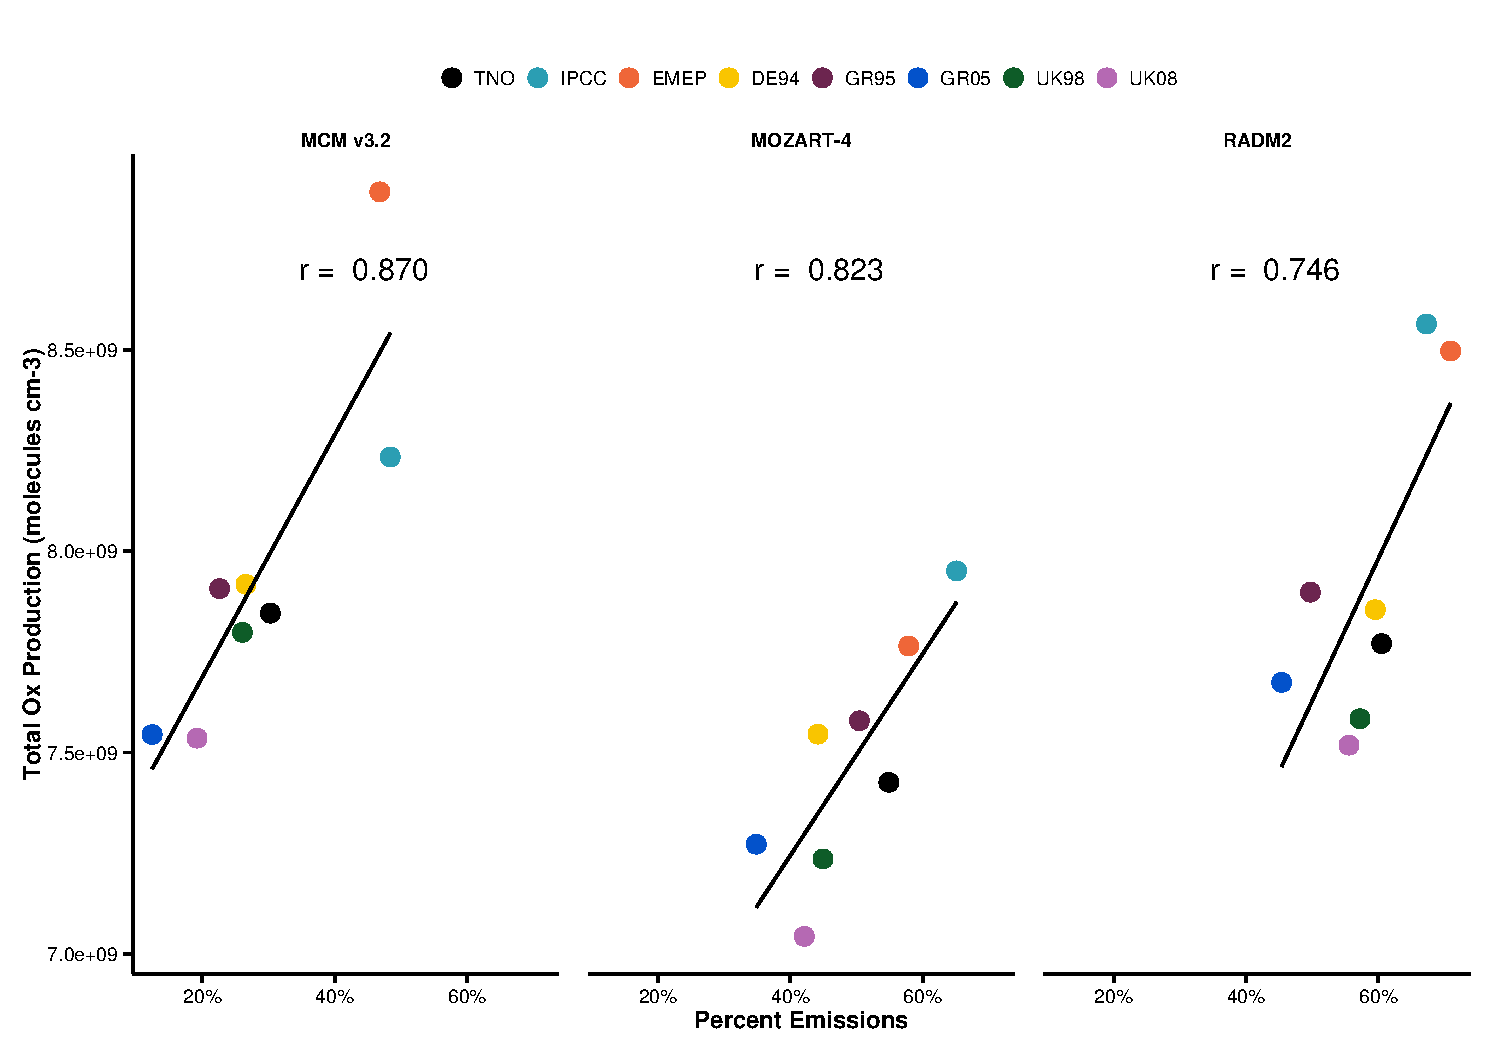
\includegraphics[height=0.90\paperheight, width = 0.98\paperwidth]{../Plotting_scripts/Ox_production_vs_type_emission_fraction_all_mechanisms}\hfil}\vfil}
    }
    \begin{frame}[plain]
    \end{frame}
}

\begin{frame}
    \frametitle{Paper Status}

    \vspace{-1cm}
    \begin{itemize}
        \item Prepared an initial draft focussing on modelling work. \vspace{5mm}
        \item Erika will be first author.  \vspace{5mm}
        \item Final paper will include more background information on comparing the different solvent sector speciations. \vspace{5mm}
        \item Submit to Atmospheric Environment by end-August.
    \end{itemize}
\end{frame}
